\documentclass[10pt,compress]{beamer}
\usepackage{amsmath}
\usepackage{cmbright}
\usepackage{url}
\usepackage{ucs}
\usepackage[utf8x]{inputenc}
\usepackage[ngerman]{babel}
\usepackage{bbm}
\usepackage{ulem}
\usepackage{multicol}
\usepackage{comment}
\usepackage{setspace}
\usepackage{color}
\usepackage{hyperref}
\usepackage{bookman}
\usepackage{wasysym}

\usetheme{Boadilla}
\setbeamertemplate{footline}%{infolines theme}

\usecolortheme{lily}
\usefonttheme{serif}
\useinnertheme{circles}
\setbeamercovered{transparent}
\beamertemplatenavigationsymbolsempty

\definecolor{darkgreen}{rgb}{0,0.5,0}

\hypersetup{
    bookmarks=true,
    unicode=true,
    pdftoolbar=true,
    pdfmenubar=true,
    pdffitwindow=false,
    pdfstartview={FitH},
    pdftitle={Ethanol -- Aufnahme und Abbau},
    pdfauthor={Michael Hartmann},
    pdfsubject={Vortrag über den zeitlichen Verlauf der Blutalkoholkonzentration im Blut},
    pdfcreator={vim},
    pdfproducer={pdflatex},
    pdfkeywords={Blutalkoholkonzentration} {Ethanol} {Aufbau} {Abbau},
    pdfnewwindow=true,
    colorlinks=true,
    linkcolor=black,
    citecolor=green,
    filecolor=magenta,
    urlcolor=darkgreen
}



\title{Ethanol -- Aufnahme und Abbau}
\institute{Kaffeeseminar}
\author{Michael Hartmann}
\date{19. Dezember 2014}


\titlegraphic{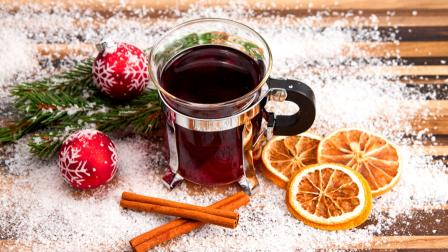
\includegraphics[scale=0.3]{images/gluehwein.jpg}}


\begin{document}

\begin{frame}
    \titlepage
\end{frame}


\frame{
    \frametitle{Überblick}
    \tableofcontents 
}


\section{Einführung}

\subsection{Motivation}
\frame {
    \frametitle{Blutalkohol}

    Widmark:
    \begin{equation}
    \nonumber
    c_\text{BAK} = \frac{m_\text{Magen}}{r\, m_\text{Körper}}
    \end{equation}

    \begin{itemize}
    \item $c_\text{BAK}$: Ethanol Konzentration im Blut
    \item $m_\text{Magen}$: Masse eingenommenen Ethanols
    \item $r$: Reduktionsfaktor; Frauen $r=0.55$, Männer $r=0.68$
    \end{itemize}

    \vfill

    Beispiel: 1l Bier (5 Volumenprozent Ethanol), 65kg, Mann
    \begin{equation}
    \nonumber
    c_\text{BAK} = \frac{\varrho V}{r\, m_\text{Körper}} = \frac{0.789 \frac{\mathrm{kg}}{\ell} \cdot 0.05 \cdot 1\ell}{0.68\cdot65\mathrm{kg}} = 0.89\permil
    \end{equation}

    \vfill
    \hfill
    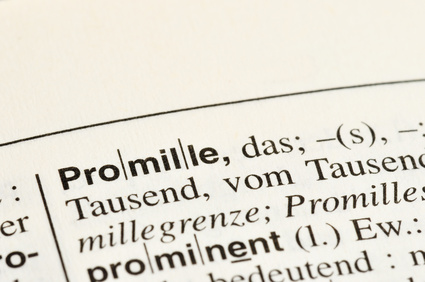
\includegraphics[scale=0.2]{images/promill.jpg}
}

\frame {
    \frametitle{offene Fragen}
    Probleme:
    \begin{itemize}
        \item Einfluss Mageninhalt?
        \item Einfluss Gewöhnung?
        \item Zeitraum der Einnahme?
        \item Wie lange dauert der Abbau? 
        \item[$\Rightarrow$] $c_\text{BAK}(t)$
    \end{itemize}

    \vfill
    \hfill
    
\includegraphics[scale=0.24]{images/patrick.jpg}
}

\subsection{Typen von Alkoholismus}
\frame {
    \frametitle{Typen von Alkoholismus}

    \begin{center}
    \begin{tabular}{cll}
    \textbf{Typ} & \textbf{Kennzeichen} & \textbf{Abhängigkeit} \\
    $\alpha$   & \small{Konflikttrinker, kein Kontrollverlust}    & \small{psychisch} \\
    $\beta$    & \small{Gelegenheitstrinker, "`Party"'}           & \small{höchstens soziokulturell} \\
    $\gamma$   & \small{Kontrollverlust, Abstinenzperioden}       & \small{psychisch, später physisch} \\
    $\delta$   & \small{Gewohnheitstrinker, kein Kontrollverlust} & \small{physisch, später psychisch} \\
    $\epsilon$ & \small{Quartalstrinker}                          & \small{zeitweilige Gefährdung}
    \end{tabular}
    \end{center}

}

\section{Modellierung}

\subsection{Abbau}


\frame {
    \frametitle{Abbau von Ethanol}

    \begin{itemize}
    \item Abbau erfolgt nahezu ausschließlich in der Leber (ca. 85-95\%)
    \item Abbaurate $\gamma$ bis $0.2\permil$ konstant und unabhängig von konsumierter Menge
    \item Abbau lässt sich durch Sport/Kaffee etc. nicht beschleunigen
    \item $\gamma$ abhängig von Gewöhnung (Toleranz) und Geschlecht
    \item typische Abbauraten ($[\gamma]=1/\mathrm{h}$):
    \vfill
    \begin{center}
    \begin{tabular}{ccc}
    \textbf{Trinkgewohnheit} & \textbf{Abbaurate $\gamma$ ($\mars$)} & \textbf{Abbaurate $\gamma$ ($\female$)} \\
    Nichttrinker             & $0.12\pm0.04$              & $0.10\pm0.03$ \\
    Gesellschaftstrinker     & $0.15\pm0.04$              & $0.13\pm0.03$ \\
    Alkoholiker              & $0.30\pm0.04$              & $0.26\pm0.03$
    \end{tabular}
    \end{center}
    \vfill
    \item DGl für für Abbau der BAK:
        \begin{equation}
        \nonumber
        \frac{\mathrm{d}}{\mathrm{d}t} c_\text{BAK} = -\gamma \Theta(c_\text{BAK})
        \end{equation}
    \end{itemize}
}

\frame {
    \frametitle{Abbau von Ethanol -- Beispiele}

    \begin{center}
    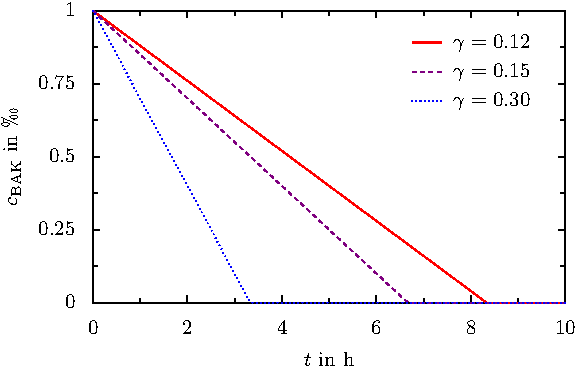
\includegraphics[scale=1.0]{images/abbau.pdf}
    \end{center}
}

\subsection{Aufnahme}

\frame {
    \frametitle{Aufnahme von Ethanol}

    \begin{itemize}
    \item Aufnahme von Ethanol i.d.R. oral
    \item im Mund/Rachenraum werden nur geringe Mengen Ethanol aufgenommen 
    \item aber: Leber wird umgangen und Wirkung ist rascher
    \item Aufnahmegeschwindigkeit ist von Konzentration abhängig
    \item schnellere Aufnahme bei süßen und kohlensäurehaltigen Getränken
    \item Ethanol verteilt sich rasch ziemlich gleichmäßig im Körper
    \item Nahrung im Magen verlangsamt die Resorption
    \vfill
    \begin{center}
    \begin{tabular}{ccc}
    \textbf{Magenfüllung} & \textbf{HWZ} (in $\mathrm{h}$) & \textbf{Resorptionsrate $\kappa$} (in $\mathrm{h}^{-1}$)\\
    leerer Magen          & $0.5$ & $1.38$ \\
    kleine Mahlzeit       & $1.0$ & $0.69$ \\
    normale Mahlzeit      & $1.5$ & $0.46$ \\
    große Mahlzeit        & $2.0$ & $0.35$
    \end{tabular}
    \end{center}
    \end{itemize}
}

\frame {
    \frametitle{Aufnahme von Ethanol}

    DGl für Masse an Ethanol im Magen:
    \begin{equation}
    \nonumber
    \frac{\mathrm{d}}{\mathrm{d}t} m_\text{Magen} = I(t) - \kappa m_{Magen}
    \end{equation}

    DGl für BAK:
    \begin{equation}
    \nonumber
    \frac{\mathrm{d}}{\mathrm{d}t} c_\text{BAK} = -\gamma + \frac{\kappa}{r \, m_\text{Körper}} m_\text{Magen} = -\gamma + \alpha m_\text{Magen}
    \end{equation}

    \vfill

    \begin{itemize}
    \item $m_\text{Magen}$: Masse Ethanol im Magen
    \item $I(t)$: Massestrom von Ethanol in den Magen; $I(t) \ge 0$
    \item $\kappa$: Resorptionsrate
    \item $\alpha=\frac{\kappa}{r\,m_\text{Körper}}$: effektive Resorptionsrate
    \end{itemize}
}

\subsection{Lösung}

\frame {
    \frametitle{Lösung}

    \begin{itemize}
    \item DGl für Masse Ethanol im Magen
    \begin{equation}
    \nonumber
    \frac{\mathrm{d}}{\mathrm{d}t} m_\text{Magen} = I(t) - \kappa m_\text{Magen}
    \end{equation}

    \item homogene Lsg
    \begin{equation}
    \nonumber
    m_\text{Magen}(t) = C e^{-\kappa t}
    \end{equation}

    \item Variation der Konstanten: $C=C(t)$
    \begin{align}
    \nonumber
    e^{-\kappa t} & \frac{\mathrm{d}}{\mathrm{d}t} C -\kappa C e^{-\kappa t} = I(t) - \kappa C e^{-\kappa t} \\
    \nonumber
    &\Rightarrow C(t) = \int_0^t \mathrm{d}t^\prime \, I(t^\prime) e^{\kappa t^\prime}
    \end{align}
    \item Lösung
    \begin{equation}
    \nonumber
    m_\text{Magen}(t) = e^{-\kappa t} \left(m_\text{Magen}(0) + \int_0^t \mathrm{d}t^\prime \, I(t^\prime) e^{\kappa t^\prime}\right)
    \end{equation}
    \end{itemize}
}

\frame {
    \frametitle{Lösung}

    \begin{itemize}
    \item DGl für BAK
    \begin{equation}
    \nonumber
    \frac{\mathrm{d}}{\mathrm{d}t} c_\text{BAK} = -\gamma + \alpha m_\text{Magen}
    \end{equation}

    \item Lösung
    \begin{equation}
    \nonumber
    c_\text{BAK}(t) = -\gamma t + \alpha \int_0^t \mathrm{d}t^\prime \, m_\text{Magen}(t^\prime) + c_\text{BAK}(0)
    \end{equation}

    \item verwendete Anfangsbedingungen
    \begin{align}
    \nonumber
    m_\text{Magen}(t=0) &= m_\text{Magen}(0) \\
    \nonumber
    c_\text{BAK}(t=0) &= c_\text{BAK}(0)
    \end{align}

    \end{itemize}
}


\section{Alkoholkurven}
\subsection{Rauschtrinken}

\frame {
    \frametitle{Rauschtrinken}

    \begin{itemize}
    \item Rauschtrinken: Aufnahme großer Mengen Alkohol in kurzer Zeit
    \item Annahme: Trinken erfolgt so schnell, dass Körper während Aufnahme kaum Ethanol abbauen kann
    \item[$\Rightarrow$] $I(t)\equiv0$
    \item[$\Rightarrow$] AB: $m_\text{Magen}(t=0) = m_0$, $c_\text{BAK}(t=0) = 0$
    \end{itemize}

    \vfill

    DGl für Masse Ethanol im Magen:
    \begin{equation}
    \nonumber
    \frac{\mathrm{d}}{\mathrm{d}t} m_\text{Magen} = - \kappa m_{Magen}
    \end{equation}

    Lösung:
    \begin{equation}
    \nonumber
    \Rightarrow m_\text{Magen}(t) = m_0 e^{-\kappa t}
    \end{equation}
}

\frame {
    \frametitle{Rauschtrinken}

    Ethanol im Magen:
    \begin{equation}
    \nonumber
    m_\text{Magen}(t) = m_0 e^{-\kappa t}
    \end{equation}

    DGl für BAK:
    \begin{equation}
    \nonumber
    \frac{\mathrm{d}}{\mathrm{d}t} c_\text{BAK} = -\gamma + \alpha m_\text{Magen} = -\gamma + \alpha m_0 e^{-\kappa t}
    \end{equation}

    Lösung:
    \begin{align}
    \nonumber
    c_\text{BAK}(t) &= \int_0^t \mathrm{d}t^\prime \left(-\gamma + \alpha m_0 e^{-\kappa t^\prime}\right) \\
    \nonumber
    &= \frac{\alpha m_0}{\kappa} \left( 1 - e^{-\kappa t} \right) - \gamma t \\
    \nonumber
    &= \frac{m_0}{r \, m_\text{Körper}} \left( 1 - e^{-\kappa t} \right) - \gamma t
    \end{align}

}

\frame {
    \frametitle{Rauschtrinken}

    \begin{itemize}
    \item Lösung
    \begin{equation}
    \nonumber
    c_\text{BAK}(t) = \frac{m_0}{r \, m_\text{Körper}} \left( 1 - e^{-\kappa t} \right) - \gamma t
    \end{equation}

    \item Maximum
    \begin{equation}
    \nonumber
    t_\text{max} = \frac{1}{\kappa} \log{\left(\frac{\kappa m_0}{\gamma r m_\text{Körper}}\right)}
    \end{equation}

    \item Beispiel: 65kg, $0.7$l Wodka, Gewohnheitstrinker, normale Mahlzeit

    \begin{center}
    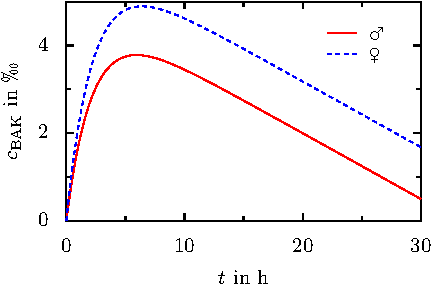
\includegraphics[scale=1.0]{images/rausch_wodka1.pdf}
    \end{center}
    \end{itemize}
}

\subsection{Wirkung von Ethanol}

\frame {
    \frametitle{Wirkung}

    \begin{center}
    \begin{tabular}{cl}
    \textbf{BAK} & \textbf{Wirkung} \\
    $0.3$    & \small{erste Gangstörung} \\
    $0.5$    & \small{negative Tiefensehschärfe, leichte motorische Störungen} \\
    $0.6$    & \small{leichte Sprachstörungen, erhöhte Reaktionszeit} \\
    $1.0$    & \small{mäßiger Rauschzustand} \\
    $1.4$    & \small{kräftiger Rausch, Grenze der akuten Vergiftung} \\
    $1.5$    & \small{Koordinations- und Gleichgewichtsstörungen} \\
    $2-3$    & \small{grobe Koordinationsstörungen, Bewusstseinstrübungen} \\
    $3-3.5$  & \small{Koma möglich} \\
    ab $3.5$ & \small{lethale Konzentration}
    \end{tabular}
    \end{center}

    \vfill
    \hfill
    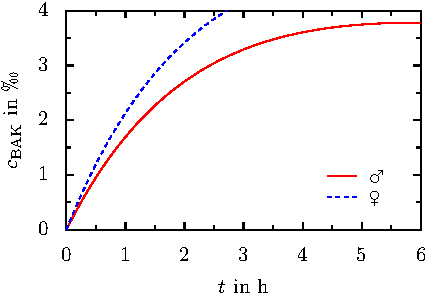
\includegraphics[scale=0.75]{images/rausch_wodka2.pdf}
}

\subsection{Konstantes Trinken}

\frame {
    \frametitle{Konstantes Trinken}

    \begin{itemize}
    \item Ethanolzuführung passiert gleichmäßig über einen Zeitraum verteilt
    \item Ethanolstrom
    \begin{equation}
    \nonumber
    I(t) = 
    \begin{cases}
        I_0 & \text{f"ur } 0 \le t \le t_E \\
        0   & \text{sonst}
    \end{cases}
    \end{equation}
    \item Anfangsbedingungen
    \begin{align}
    \nonumber
    c_\text{BAK}(t=0)   &= 0 \\
    \nonumber
    m_\text{Magen}(t=0) &= 0
    \end{align}
    \end{itemize}
}

\frame {
    \frametitle{Konstantes Trinken}

    Bsp: Mann, 65kg, Gewohnheitstrinker, $0.7$l Wodka, normale Mahlzeit

    \begin{center}
    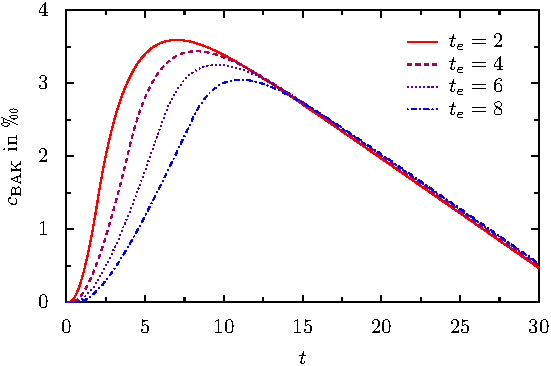
\includegraphics[scale=1]{images/wodka_konst.pdf}
    \end{center}
}

\frame {
    \frametitle{Konstantes Trinken}

    Bsp: Mann, 65kg, Gewohnheitstrinker, 6 Bier, normale Mahlzeit

    \begin{center}
    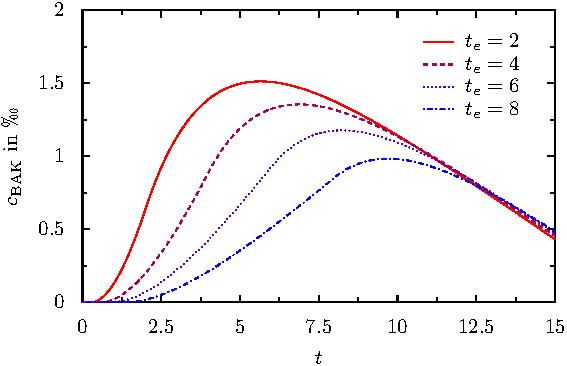
\includegraphics[scale=1]{images/bier.pdf}
    \end{center}
}

\subsection{Zwei Maß Bier auf dem Oktoberfest}

\frame {
    \frametitle{"`Nach zwei Maß kann man noch Autofahren..."'}

    Bsp: Mann, 65kg, Gewohnheitstrinker, normale Mahlzeit

    \begin{center}
    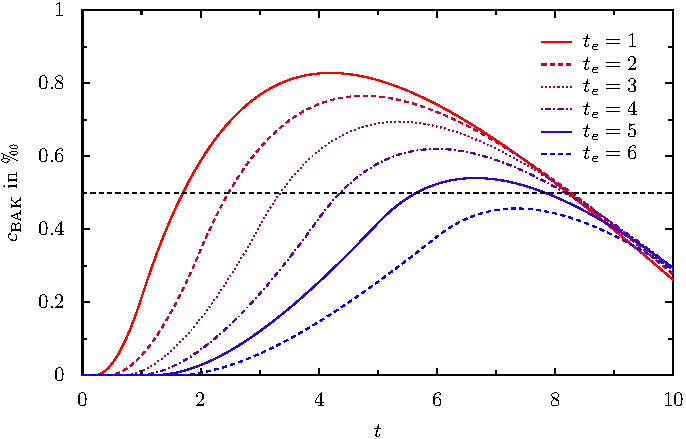
\includegraphics[scale=0.9]{images/bier_auto1.pdf}
    \end{center}
}

\frame {
    \frametitle{"`Nach zwei Maß kann man noch Autofahren..."'}

    Bsp mit Schweinshaxe: große Mahlzeit

    \begin{center}
    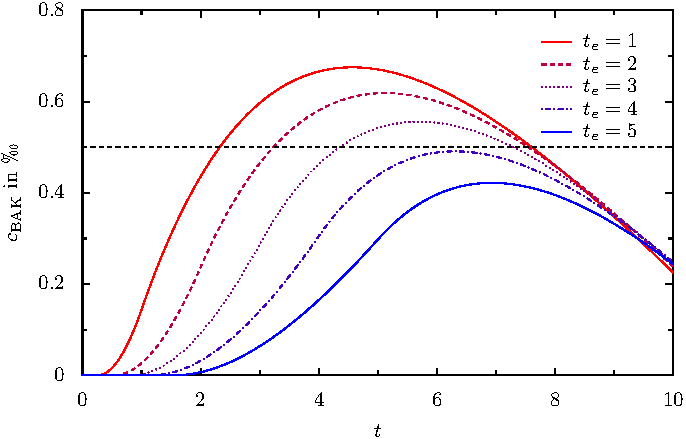
\includegraphics[scale=0.9]{images/bier_auto2.pdf}
    \end{center}
}

\section{Zusammenfassung}
\frame {
    \frametitle{Zusammenfassung}

    \begin{itemize}
    \item Ethanol gelangt oral in den Magen
    \item Ethanol gelangt von dort ins Blut -- Geschwindigkeit ist proportional zur Menge im Magen
    \item Abbau erfolgt bis etwa $0.2\permil$ mit konstanter Geschwindigkeit
    \item Maximum der BAK ist zeitlich deutlich verzögert
    \item Konzentration im Gehirn durch Blut-Hirn-Schranke weiter verzögert
    \end{itemize}

    Na dann: Prost Neujahr!

    \vfill
    \hfil
    \hfil
    \hfil
    \hfil
    \hfil
    \hfil
    \hfil
    \hfil
    \hfil
    \hfil
    \hfil
    \hfil
    \hfil
    \hfil
    \hfil
    \hfil
    \hfil
    \hfil
    \hfil
    \hfil
    \hfil
    \hfil
    \hfil
    \hfil
    \hfil
    \hfil
    \hfil
    \hfil
    \hfil
    \hfil
    \hfil
    \hfil
    \hfil
    \hfil
    \hfil
    \hfil
    \hfil
    \hfil
    \hfil
    \hfil
    \hfil
    \hfil
    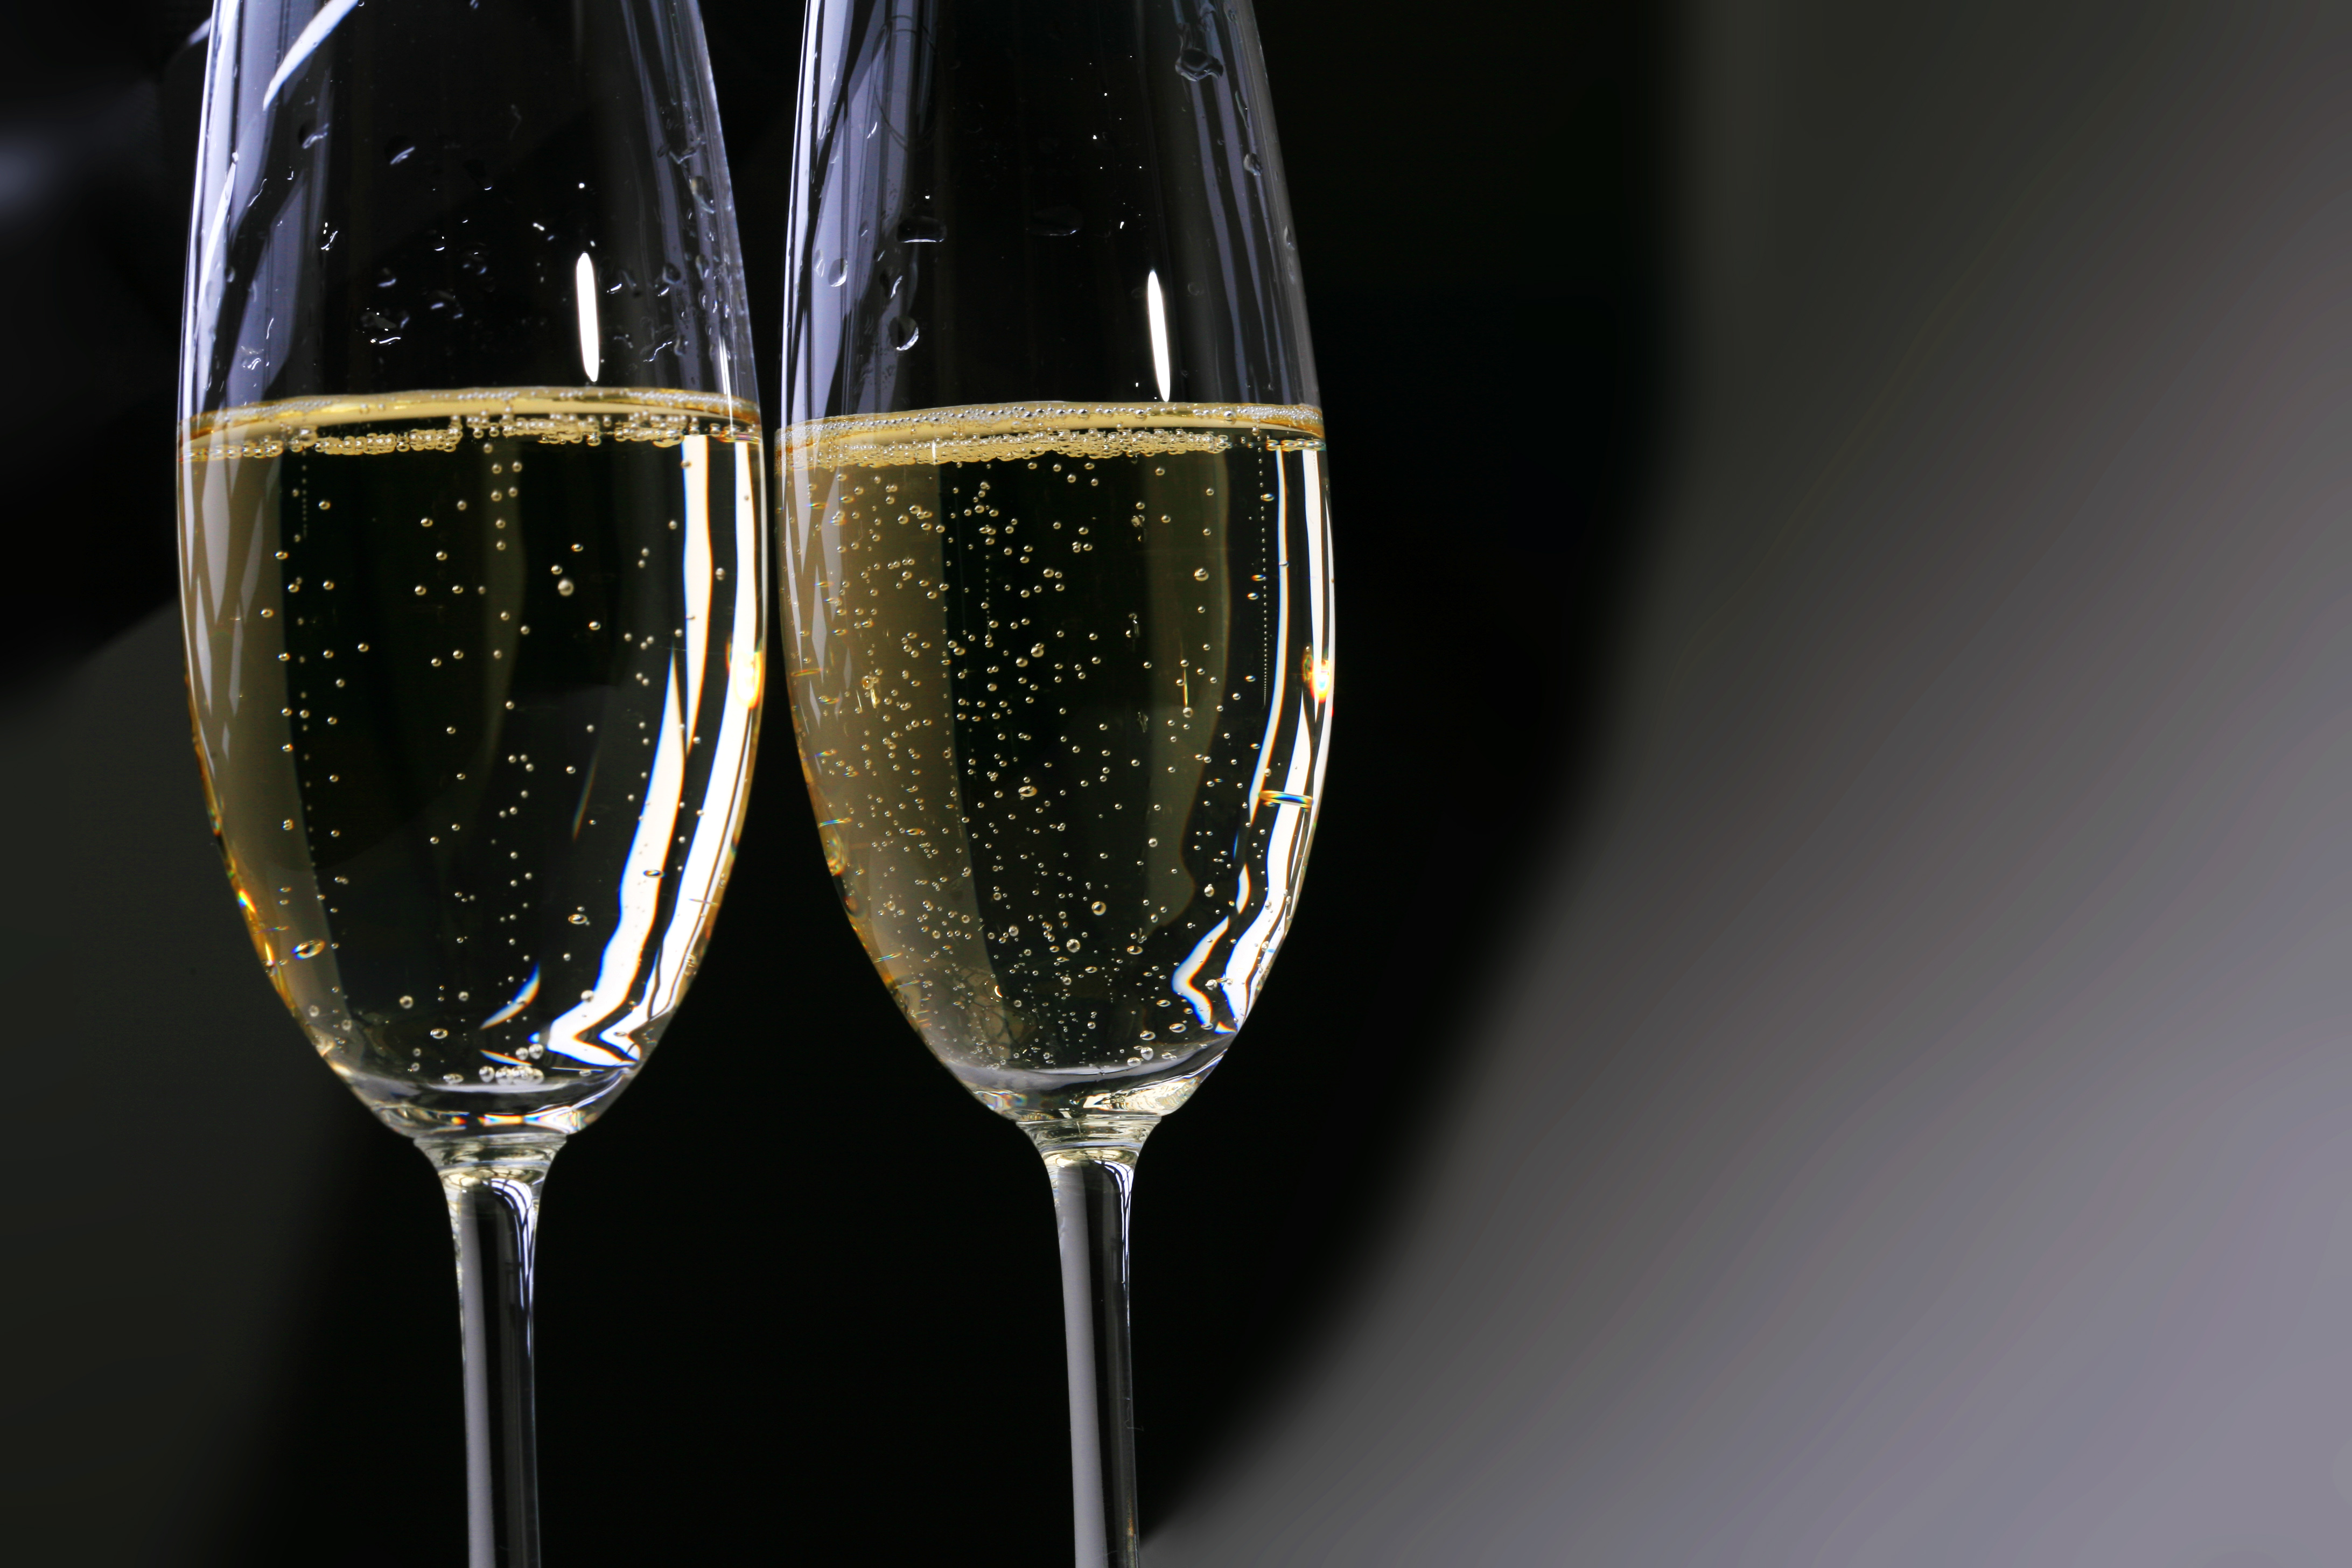
\includegraphics[scale=0.023]{images/neujahr.jpg}
}

\end{document}
